\documentclass[a4paper,12pt]{article}
\usepackage[english,ukrainian,russian]{babel}
\linespread{1}
\usepackage{ucs}
\usepackage[utf8]{inputenc}
\usepackage[T2A]{fontenc}
\usepackage[paper=portrait,pagesize]{typearea}
\usepackage{amsmath}
\usepackage{bigints}
\usepackage{amsfonts}
\usepackage{graphicx}
\usepackage{amssymb}
\usepackage{cancel}
\usepackage{gensymb}
\usepackage{multirow}
\usepackage{rotate} 
\usepackage{pdflscape}
\usepackage{bigstrut}
\usepackage[pageanchor]{hyperref}
\usepackage{chngpage}
\newcommand{\dx}{\textbf{d}x}
\newcommand{\dt}{\textbf{d}t}
\newcommand{\du}{\textbf{d}u}
\newcommand{\dv}{\textbf{d}v}
\newcommand{\dy}{\textbf{d}y}
\newcommand{\ds}{\textbf{d}s}
\newcommand{\dz}{\textbf{d}z}
\newcommand{\arch}{\textrm{arcch}}
\newcommand{\arsh}{\textrm{arcsh}}
\newcommand{\dint}{\displaystyle\int}
\newcommand\tab[1][1cm]{\hspace*{#1}}
\newcommand{\dsum}{\displaystyle\sum}
\usepackage[left=20mm, top=20mm, right=15mm, bottom=15mm, nohead, nofoot]{geometry}
\usepackage{verbatim}

\usepackage{color} %% это для отображения цвета в коде
\usepackage{listings} %% собственно, это и есть пакет listings
\usepackage{caption}
\definecolor{gray}{RGB}{117, 117, 117}
\definecolor{dkgreen}{rgb}{0,0.6,0}
\definecolor{gray}{rgb}{0.5,0.5,0.5}
\definecolor{mauve}{rgb}{0.58,0,0.82}
\DeclareCaptionFont{white}{\color{white}} %% это сделает текст заголовка белым
%% код ниже нарисует серую рамочку вокруг заголовка кода.
\DeclareCaptionFormat{listing}{\colorbox{gray}{\parbox{\textwidth}{#1#2#3}}}
\captionsetup[lstlisting]{format=listing,labelfont=white,textfont=white}
\renewcommand{\lstlistingname}{Листинг}


\begin{document}
	\begin{center}
		%\vspace*{0,1cm}
		{\Large \bfseries \textsc{Лабораторна робота №1}}\\
		\hrulefill\\
		\Large \textsc{ФІ-12 Завалій Олександр\\ Варіант №5}
	\end{center}
	\begin{center}
		\section*{\bfseries{Завдання}}
	\end{center} 
	\textbf{Предметна область:} \\
	Навчально-методичне управління (облік площі приміщень). \\
	\textbf{Основні предметно-значущі сутності:} \\
	Приміщення, Підрозділи. \\
	\textbf{Основні предметно-значущі атрибути сутностей:}
	\begin{enumerate}
		\item[-] \textbf{Приміщення}: назва або номер приміщення, вид приміщення (аудиторія, кабінет і т.п.), площа, кількість посадочних місць, підрозділ. 
		\item[-] \textbf{Підрозділи}: назва, вид підрозділу.
	\end{enumerate}
	\textbf{Основні вимоги до функцій системи:}
	\begin{enumerate}
		\item[-] Вибрати назви або номери приміщень за підрозділами;
		\item[-] Підрахувати загальну площу навчальних аудиторій по приміщеннях і в цілому по навчальному закладу;
		\item[-] Підрахувати загальну кількість посадочних місць для співробітників по підрозділам.
	\end{enumerate}
	\textbf{Тригери:}
	\begin{enumerate}
		\item На видалення запису з таблиці «Приміщення». Якщо для приміщення зазначено підрозділ, заборонити видалення запису.
		\item Створити представлення «Аудиторії» з полями «код приміщення», «назва приміщення», «підрозділ», в яку повинні входити приміщення виду «Аудиторія». Оновлювати представлення «Аудиторії».
	\end{enumerate}
	\textbf{Процедура:}\\
	Процедура повинна повертати кількість приміщень для зазначеного підрозділу. \\
	\begin{center}
		\textbf{Завдання для лабораторної роботи}
	\end{center}
	\begin{enumerate}
		\item Вибрати у відповідності до списку групи свій варіант завдання. Проаналізувати опис предметної області. Створити необхідні таблиці.
		\item За допомогою SSMS побудувати ER-діаграму створеної бази даних.
	\end{enumerate}

\newpage
	\begin{center}
		\section*{\bfseries{Реалізація завдання}}
	\end{center}

	\lstset{%
		language=SQL,                 % выбор языка для подсветки (здесь это С)
		basicstyle=\small\sffamily, % размер и начертание шрифта для подсветки кода
		%numbers=left,               % где поставить нумерацию строк (слева\справа)
		numberstyle=\tiny,           % размер шрифта для номеров строк
		stepnumber=1,                   % размер шага между двумя номерами строк
		numbersep=5pt,                % как далеко отстоят номера строк от подсвечиваемого кода
		backgroundcolor=\color{white}, % цвет фона подсветки - используем \usepackage{color}
		showspaces=false,            % показывать или нет пробелы специальными отступами
		showstringspaces=false,      % показывать или нет пробелы в строках
		showtabs=false,             % показывать или нет табуляцию в строках
		frame=single,              % рисовать рамку вокруг кода
		tabsize=2,                 % размер табуляции по умолчанию равен 2 пробелам
		captionpos=t,              % позиция заголовка вверху [t] или внизу [b] 
		breaklines=true,           % автоматически переносить строки (да\нет)
		breakatwhitespace=false, % переносить строки только если есть пробел
		escapeinside={\%*}{*)}   % если нужно добавить комментарии в коде
	}

	
	\begin{verbatim}
		CREATE DATABASE Educational_and_methodological_management
		GO
		
		USE Educational_and_methodological_management
		
		CREATE TABLE Subdivision(
		Subdivision_id INT IDENTITY PRIMARY KEY,
		Subdivision_name VARCHAR(50) UNIQUE NOT NULL,
		Subdivision_type VARCHAR(50) NOT NULL
		);
		
		CREATE TABLE Type_of_room(
		Type_of_room_id INT IDENTITY PRIMARY KEY,
		Type_of_room_name VARCHAR(50) UNIQUE NOT NULL
		);
		
		CREATE TABLE Type_of_seats(
		Seats_id INT IDENTITY PRIMARY KEY,
		Type_of_seats VARCHAR(50) UNIQUE NOT NULL,
		Seats_material VARCHAR(50) NOT NULL
		); 
		
		CREATE TABLE Rooms(
		Room_number INT IDENTITY PRIMARY KEY,
		Id_Type_of_room INT NOT NULL,
		Area INT NOT NULL,
		Amount_seats INT NOT NULL,
		Type_of_seats_id int, 
		Id_subdivision INT,
		CONSTRAINT Error_subdivision_id FOREIGN KEY (Id_subdivision) 
		REFERENCES Subdivision (Subdivision_id) ON DELETE SET NULL,
		CONSTRAINT Error_id_type_of_room FOREIGN KEY (Id_type_of_room) 
		REFERENCES Type_of_room (Type_of_room_id) ON DELETE CASCADE,
		CONSTRAINT Error_type_of_seats_id FOREIGN KEY (Type_of_seats_id) 
		REFERENCES Type_of_seats (Seats_id) ON DELETE SET NULL
		);
		

		Commands completed successfully.
		Completion time: 2022-10-04T19:41:34.2005860+03:00
	\end{verbatim}

	
	\begin{figure}[h!]
		\begin{center}
			\begin{minipage}[h]{0.9\linewidth}
			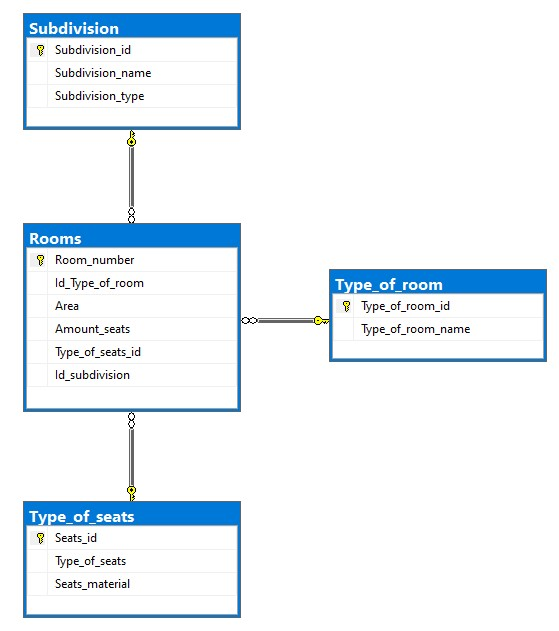
\includegraphics[width=1\linewidth]{Entity relationship diagram.jpg}
		\end{minipage}
		\end{center}
		\caption{Entity relationship diagram}
	\end{figure}
	
\end{document}